%%%%%%%%%%%%%%%%%%%%%%%%%%%%%%%%%%%%%%%%%%%%%%%%%%%%%%%%%%%%%%%%%%%
%                     THESIS PRESENTATION
%				   PATIENT TRACKING TO REDUCE
%                       INFECTION SPREAD
%				    July, 2015 - May, 2016
%%%%%%%%%%%%%%%%%%%%%%%%%%%%%%%%%%%%%%%%%%%%%%%%%%%%%%%%%%%%%%%%%%%
\documentclass{beamer}

\usepackage{graphicx} 
\graphicspath{{./img/}}

% put all the other packages here:
\usepackage{mystyle}

\title[Thesis Presentation]{Outpatient Tracking to Reduce Cross Infection}
\subtitle{Progress Report}
\author{Karthik Jayaraman}
\institute{University of New South Wales}
\date{\nth{29} October, 2015}

\begin{document}

\begin{frame}
  \titlepage
\end{frame}

% Uncomment these lines for an automatically generated outline.
%\begin{frame}{Outline}
%  \tableofcontents
%\end{frame}

\section{Introduction} \label{sec:intro}% 1-2 mins

% background + motivation for work
\subsection{Background} \label{ssec:intro_bg}
\begin{frame}{Background}

	\begin{figure}[t]
		\includegraphics<4-4>[width=\textwidth,height=0.8\textheight,keepaspectratio]{acute-cystic-fibrosis}
	\end{figure}

  \begin{itemize}
  \item<1-3,5| alert@+> 200,000 hospital acquired infections (HAIs) occur annually in Australia.
  \item<2-3,5| alert@+> In-patient care vs out-patient care
  \item<3-3,5| alert@+> Cystic Fibrosis (CF) is a genetic condition that primarily affects the lungs.
  \item<5-| alert@5> CF health care delivery has moved to out-patient environments.
  \end{itemize}
  
\end{frame}

\subsection{Research Outline} \label{ssec:intro_research}
\begin{frame}{Research Outline}

	\begin{block}<2->{Hypothesis}
    	Our hypothesis is that patient encounters can be tracked using lightweight indoor localisation technologies allowing for interventions to improve patient flow, reduce patient contact, and reduce HAIs.
    \end{block}
    
    \begin{block}<3->{Aim}
    	Identify areas of potential cross infection in the hospital out-patient environment.
    \end{block}
    
\end{frame}

\subsection{Scope} \label{ssec:intro_scope}
\begin{frame}{Scope}

	\begin{itemize}[<+-| alert@+>]
      \item Android smart-phone
      	\begin{itemize}
			\item presence of low cost embedded sensors in smart-phones
            \item ubiquity and support available for android development
            \item ease and simplicity involved in implementation
	   	\end{itemize}
      \item Air-borne infection transmission among CF patients
      \item SNA focused on disease transmission and control
  	\end{itemize}

\end{frame}

\subsection{Objectives} \label{ssec:intro_obj}
\begin{frame}{Objectives}
	
	\begin{itemize}[<+-| alert@+>]
		\item Investigation into an accurate and scalable indoor RTLS approach for tracking patient movements.
		\item Development of a smart-phone application to accurately track the position of the CF patient indoors.
		\item Development of algorithms to identify high risk areas for CF patients in the hospital out-patient environment.
		\item Implementation and testing of the software system to identify areas of improvement and practicality of system.
	\end{itemize}
	
\end{frame}

\section{Literature Review} \label{sec:litRev} % 2-3 mins

\subsection{Purpose} \label{ssec:litRev_purpose}
\begin{frame}{Purpose}

	\begin{itemize}[<+-| alert@+>]
      \item conduct a study of current technology and systems
      \item Main  components of thesis:
      	\begin{itemize}
			\item real time indoor positioning to track patients
            \item social network analysis (SNA) to identify high risk areas
	   	\end{itemize}
       \item RTLS systems in hospitals
       \item Indoor positioning technologies
       \item SNA in disease transmission and control 
  	\end{itemize}

\end{frame}

\subsection{RTLS in Hospitals} \label{ssec:litRev_rtls}
\begin{frame}{Real Time Location Systems (RTLS) in Hospitals}

    \begin{figure}[t]
      \includegraphics<3-3>[width=\textwidth,height=0.8\textheight,keepaspectratio]{rtls}
	\end{figure}

	\begin{itemize}
      \item<1-2,4-5| alert@+> RTLS is an integral part of the health care industry
      \item<2-2,4-5| alert@+> RTLS components
      \item<4-| alert@4> Used in monitoring and workflow improvements
      \item<5-| alert@5> No consistent RTLS system
  	\end{itemize}

\end{frame}

\subsection{Indoor Localisation} \label{ssec:litRev_inLocal}
\begin{frame}{Indoor Localisation}
    
    \begin{itemize}[<+-| alert@+>]
      \item Pedestrian Dead Reckoning (PDR)
      \item Direct Sensing
      \item Triangulation
      \item Pattern Recognition
  	\end{itemize}

\end{frame}

\subsubsection{PDR} \label{sssec:litRev_inLocal_PDR}
\begin{frame}{Pedestrian Dead Reckoning (PDR)}

	\includegraphics<4>[width=\textwidth,height=0.8\textheight,keepaspectratio]{step}

	\begin{itemize}[<+-| alert@+>]
      \item Dead reckoning systems specific to pedestrians
      \item Generally consists of a step-heading cycle:
      \begin{itemize}
		\item Sample sensor recordings for specific timeframe
        \item Detect Step and estimate step size
        \item Estimate step heading
	  \end{itemize}
      \item Infrastructure free
      \item Error accumulation
  	\end{itemize}

\end{frame}

\subsubsection{Direct Sensing Technologies} \label{sssec:litRev_inLocal_ds}
\begin{frame}{Direct Sensing Technologies}

	\begin{itemize}[<+-| alert@+>]
      \item Infrared (IR)
      \item Radio Frequency Identifier Description (RFID)
      \item Ultrasound Identification (USID)
      \item Wireless Networks (WLAN)
  	\end{itemize}

\end{frame}

\subsubsection{Positioning Techniques} \label{sssec:litRev_inLocal_posTech}
\begin{frame}{Positioning Techniques}

	\begin{itemize}[<+-| alert@+>]
    \item Triangulation    
        \begin{itemize}
          \item Tags are installed using direct sensing technologies.
          \item Position of the tags are known and used in the triangulation method
        \end{itemize}
        
    \item Computer Vision    
        \begin{itemize}
            \item Offline Stage - capture images of various location / physical landmarks
            \item Online Stage - compare current captured image to image database
        \end{itemize}

    \item Fingerprinting   
        \begin{itemize}
            \item Offline Stage - sampling locations to build a radio map
            \item Online Stage - compare current recorded RSSI to radio map.
        \end{itemize}

  	\end{itemize}

\end{frame}

%\subsection{Social Network Analysis} \label{ssec:litRev_sna}
%\begin{frame}{Social Network Analysis}
%\end{frame}
\section{Method} \label{sec:method} % 2-3 mins

\subsection{Pedestrian Dead Reckoning} \label{ssec:method_PDR}
\begin{frame}{Pedestrian Dead Reckoning}
	
	\includegraphics<9>[width=\textwidth,height=0.8\textheight,keepaspectratio]{heading}
	\centering
	\only{\\$\omega_{compass} = \frac{\psi_{compass}(t_{k} + \Delta t) - \psi_{compass}(t_k)}{\Delta t}$}<9>
	
		\includegraphics<10>[width=\textwidth,height=\textheight,keepaspectratio]{pdrFlow}
		\only{ \begin{equation*}
			\begin{aligned}
			\boldsymbol{x}= 
			\begin{bmatrix}
			x\\
			y 
			\end{bmatrix}
			=
			\begin{bmatrix}
			x + s\sin(\theta)\\
			y + s\cos(\theta)
			\end{bmatrix}
			\end{aligned}
			\end{equation*}}<10>

	\begin{itemize}[<1-8>]
    	\item<1-8 | alert@+> Step detection
        	\begin{itemize}
              \item<2-8 | alert@+> Combine acceleration along all three axes 
              \item<3-8| alert@+> Step detection based on peak length, zero-crossing
        	\end{itemize}
        	
        \item<4-8| alert@+> Step length estimation      
        	\begin{itemize}
              \item<5-8| alert@+> Constant value
              \item<6-8| alert@+> Weinberg approach:  $\sqrt[4]{A_{max} - A_{min}} \times n \times k$
              \item<7-8| alert@+> Scarlet approach:  $k \times \sqrt[3]{\frac{\sum_{k=1}^{N} \lvert a_k\rvert}{N}}$
        	\end{itemize}
        	
        \item<8-8| alert@+> Heading estimation
  	\end{itemize}
  	
\end{frame}

\subsection{Hybrid PDR} \label{ssec:method_hybrid}
\begin{frame}{Hybrid PDR}
\begin{itemize}[<+-| alert@+>]
    \item Bayesian Filtering    
        \begin{itemize}
	      \item Kalman Filter  
          \item Particle Filter: 
          \begin{equation*}
          \begin{aligned}
          \boldsymbol{x}_{t}^{i} = 
          \begin{bmatrix}
          x_{t}^{i}\\
          y_{t}^{i} 
          \end{bmatrix}
          =
          \begin{bmatrix}
          x_{t-1}^{i} + s_{t}^{i}\sin(\theta^{i}_{t})\\
          y_{t-1}^{i} + s_{t}^{i}\cos(\theta^{i}_{t})
          \end{bmatrix}
          \end{aligned}
          \end{equation*}
        \end{itemize}
        
    \item Error Correction with Direct Sensing Technology   
        \begin{itemize}
            \item Bluetooth Beacons with known positions scattered through the map
        \end{itemize}

  	\end{itemize}

\end{frame}
\section{Results} \label{sec:results}% 2-3 mins

\subsection{Step Detection} \label{ssec:results_stepD}
\begin{frame}{Step Detection}
	
	\begin{figure}
		\centering
		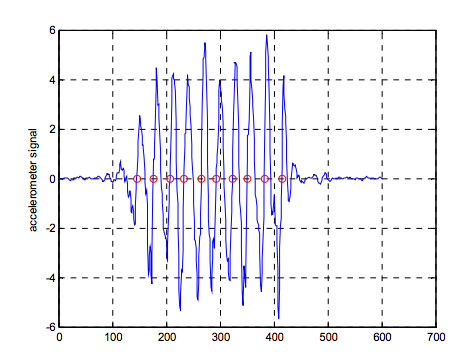
\includegraphics[scale = 0.4]{stepD}
	\end{figure}

\end{frame}

\subsection{Heading Estimation} \label{ssec:results_headinEst}
\begin{frame}{Heading Estimation}
	
		\begin{figure}
			\centering
			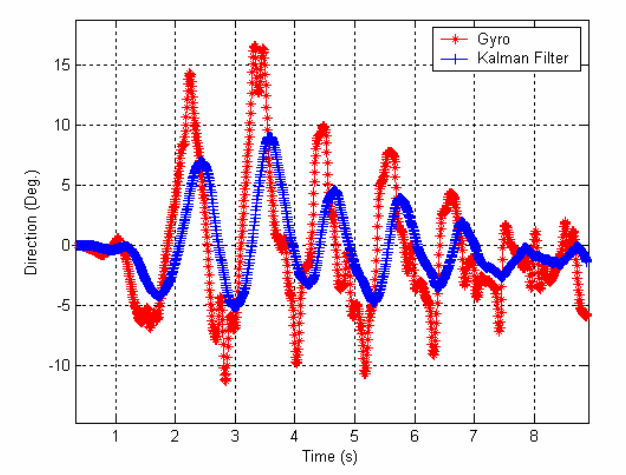
\includegraphics[scale = 0.4]{headingEst}
		\end{figure}

\end{frame}

\subsection{Map Matching} \label{ssec:results_mapM}
\begin{frame}{Map Matching}
	
	\begin{figure}
		\centering
		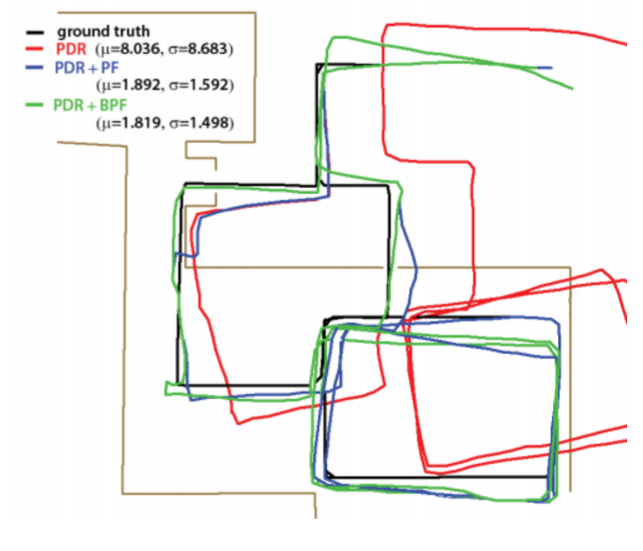
\includegraphics[scale = 0.4]{mapM}
	\end{figure}
	
\end{frame}
\section{Conclusion} \label{sec:conclusion} % 1-2 mins

\subsection{Summary} \label{ssec:conclusion_summary}
\begin{frame}{Summary}
	
	\begin{itemize}[<+-| alert@+>]
		\item Identified Research Aims
		\item Conducted literature Review
		\item PDR Implementation
		\item Preliminary experimentation
	\end{itemize}

\end{frame}

\subsection{Future Work} \label{ssec:conclusion_future}
\begin{frame}{Future Work}
	
	\begin{itemize}[<+-| alert@+>]
		\item PDR Modifications and Improvements
		\begin{itemize}
			\item Testing other algorithms for Step-Heading Cycle
			\item Modifications to the particle filter - more particles, backtracking particle filter
			\item Further experimentation and Testing
		\end{itemize}
		\item Software Design Approach
		\begin{itemize}
			\item Waterfall Model to Agile Model
			\item User Interface creation
		\end{itemize}
		\item Social Network Analysis
		\begin{itemize}
			\item Literature Review
			\item Implementation approach
		\end{itemize}
		\item Field Testing
	\end{itemize}
	

\end{frame}

\end{document}
